\documentclass[tikz]{standalone}
\usepackage[utf8]{inputenc}
\usetikzlibrary{calc,intersections}

\definecolor{DarkBlue}{rgb}{0.0,0.0,0.6}

\begin{document}

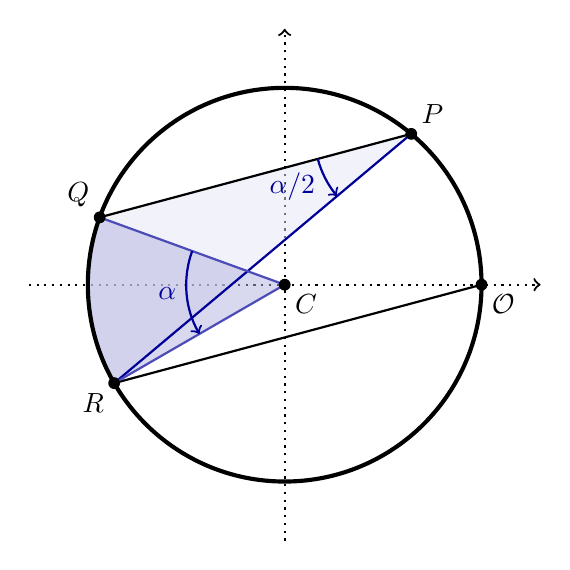
\begin{tikzpicture}[thick,scale=2.5]
\def\ptsize{.03}
\newcount\Pangle
\newcount\Qangle
\newcount\Rangle
\Pangle=50
\Qangle=160
\Rangle=\Pangle
\advance\Rangle by \Qangle
\draw[->,dotted] (-1.3, 0) -- (1.3,0);
\draw[->,dotted] (0,-1.3) -- (0,1.3);

\coordinate[label=below right:$\mathcal{O}$] (inf) at (1,0);
\coordinate[label=above right:$P$] (P) at (\number\Pangle:1);
\coordinate[label=above left:$Q$] (Q) at (\number\Qangle:1);
\coordinate[label=below left:$R$] (R) at (\number\Rangle:1);
\coordinate[label=below right:$C$] (C) at (0,0);

\fill[DarkBlue!10,opacity=.5] (P) -- (Q) arc (\number\Qangle:\number\Rangle:1) -- cycle;
\fill[DarkBlue!30,opacity=.5] (C) -- (Q) arc (\number\Qangle:\number\Rangle:1) -- cycle;

\path[draw,name path=circ,line width=1.5pt] (0,0) circle (1);

\draw (P) -- (Q);
\draw (inf) -- (R);

\draw[line width=.8pt,DarkBlue] (P) -- (R);
\draw[line width=.8pt,DarkBlue!70] (Q) -- (C) -- (R);
\draw[DarkBlue,line width=.8pt,->] ($(C)!.5!(Q)$) arc (\number\Qangle:\number\Rangle:.5) node[midway,left] {$\alpha$};

\draw[DarkBlue,line width=.8pt,->] ($(P)!.3!(Q)$) arc (195:220:.491) node[midway,left,yshift=-3pt] {$\alpha/2$};

\fill (inf) circle (\ptsize);
\fill (P) circle (\ptsize);
\fill (Q) circle (\ptsize);
\fill (R) circle (\ptsize);
\fill (C) circle (\ptsize);

\end{tikzpicture}

\end{document}